\section{Background}
\label{sec:background}
{\color{red}---Catchy first sentence.}\newline
\textit{Machine learning} aims to infer generally valid relationships from a finite set of training data and apply those learned relations to new data \cite{domingos2012few, kotsiantis2007supervised}. While some problems can be solved by manually encoding explicit rules, others require a different approach as explicit decision-making does not deliver highly accurate results \cite{burrell2016machine}. Determining a student's grade in a multiple choice test can be solved by explicitly encoding mathematical rules, yet deciding whether the tonality of a text is positive or negative needs more than a simple rule set to function accurately \cite{melville2009sentiment}. The datasets needed to train machine learning models are often large and represented in a high-dimensional feature space, which makes it impossible for a human to carry out the learning task like a machine can. However, machines can be used to extend the cognitive capabilities of humans when working together on those learning tasks. \cite{ventocilla2018taxonomy} describes the fruitful collaboration between human and machine as \textit{augmented intelligence}.\newline
{\color{red}---Narrowing topic to decision-making (supervised classification) and discriminative algorithms and define "decision" as output from ML systems}


%------------------------------------------------------------------
\subsection{Interpretability in AI}
Humans cooperating with machines need to understand the principles of the method that is employed - a property referred to as \textit{transparency} \cite{kotsiantis2007supervised}. \textit{Opacity}, the direct opposite of transparency \cite{lipton2016mythos}, is a major problem for augmented intelligence. Although opacity can be used voluntarily as a means to self-protection and censorship, it also arises involuntarily due to missing technical expertise and failed human intuition and cognitive abilities \cite{burrell2016machine}.\newline
On the application-side of machine learning systems, the question of transparency brings up the notion of \textit{interpretability}. Interpretability refers to how well a ``typical classifier generated by a learning algorithm" can be understood \cite{kotsiantis2007supervised}, as compared to the theoretical principle of the method. That is, an interpretable machine learning system is either inherently interpretable, meaning that its operations and result patterns can be understood by a human \cite{biran2017explanation, ventocilla2018taxonomy}, or it is capable of generating descriptions understandable to humans \cite{gilpin2018explaining}. It is also possible to equip a system retrospectively with interpretability by adding a proxy model capable of approximating the original system's behaviour while being comprehensible for humans \cite{guidotti2018survey}. Using an interpretable system as a human means being enabled to make inferences about underlying data \cite{ventocilla2018taxonomy}.\newline
\cite{guidotti2018survey} assigns ten desired dimensions to interpretable machine learning systems:
\begin{itemize}
	\item \textit{Scope}: Global interpretability (understanding the model and operations) and local interpretability (understanding what brought about a single decision)
	\item \textit{Timing}: Time scope available in the application use case for a target user to understand 
	\item \textit{Prior knowledge}: Level of expertise of target user
	\item \textit{Dimensionality}: Size of the model and the data
	\item \textit{Accuracy}: Target accuracy of the system while maintaining interpretability
	\item \textit{Fidelity}: Accuracy of explanation vs. accuracy of model
	\item \textit{Fairness}: Robustness against automated discrimination and ethically challenging biases in data
	\item \textit{Privacy}: Protection of sensible and personal data
	\item \textit{Monotonicity}: Level of monotonicity in relations of input and output (human intuition is largely monotonic)
	\item \textit{Usability}: Efficiency, effectiveness, and joy of use
\end{itemize}
In the context of interpretability for machine learning systems, the terms \textit{understandability}, \textit{comprehensibility}, \textit{explainability}, and \textit{justification} are often mentioned in literature. In this paper, we adopt the definition of \cite{ruping2006learning}. \textit{Understandability}, \textit{accuracy} of the explanation, and \textit{efficiency} of the explanation together form \textit{interpretability}. \textit{Explainability} is a synonym of \textit{comprehensibility} \cite{weihs2003combining}, which is also synonymic to \textit{understandability} \cite{bibal2016interpretability} and therefore an aspect of interpretability, showing the reasons for the system's behaviour \cite{gilpin2018explaining}. Figure \ref{fig:definitions} gives an overview over these terms. Finally, \textit{justification} refers to the evidence for why a decision is correct, which does not necessarily include the underlying reasons and causes \cite{biran2017explanation}.\newline
\begin{figure} [h]
	\centering
	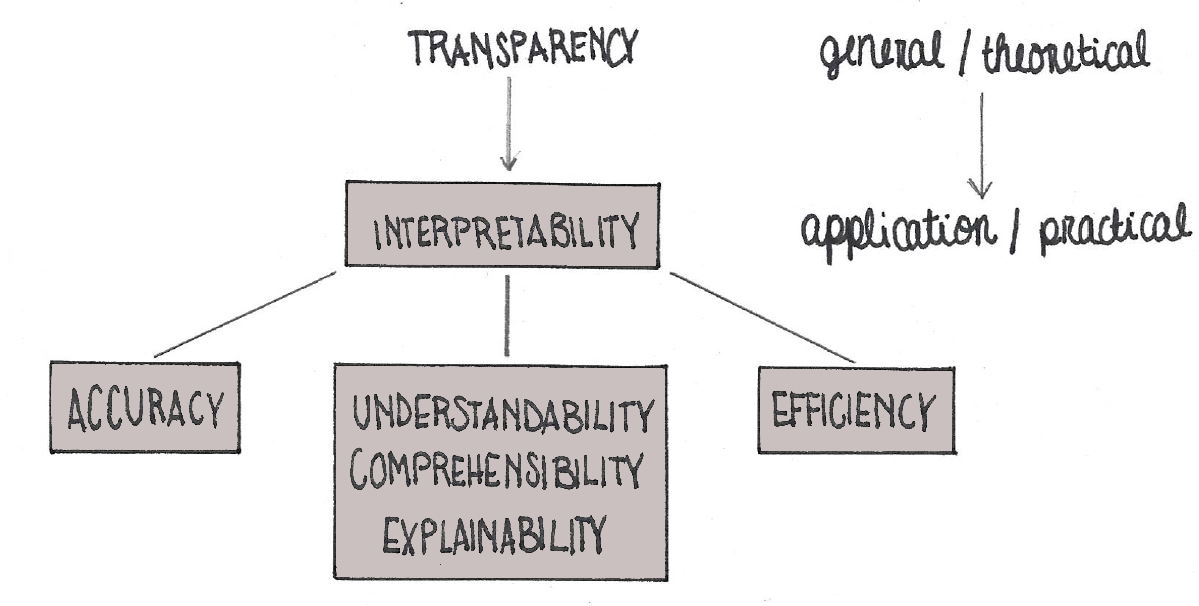
\includegraphics[width=0.7\linewidth]{img/definitions2}
	\caption{Relation of terms connected to interpretability}
	\label{fig:definitions}
\end{figure}
If the human cognition is augmented by a machine learning system, talking about interpretability should also include discussing the interpretability of the human in the loop. \cite{lipton2016mythos} argues that human behaviour is often mistakenly identified as interpretable because humans can explain their actions and beliefs. Yet the actual operations of the human brain remain opaque, which contradicts the concept of interpretability \cite{lipton2016mythos}. If human reasoning is taken as a point of reference for the discussion of algorithmic interpretability, the absence of verifiability should be taken into account. Human interpretability, however, is not the focus of this paper and will therefore not be discussed in more detail here.\newline





%------------------------------------------------------------------
\subsection{Need for Explainability in AI}
\label{subsec:explainability}
A subfield of artificial intelligence research revolves solely around the explainability of intelligent systems: \textit{xAI}, explainable artificial intelligence, for the purpose of enabling communication with agents about their reasoning \cite{hendricks2018generating}. xAI systems face a trade-off challenge as their explanation has to be complete and interpretable at the same time \cite{gilpin2018explaining}. The attention span and cognitive abilities of humans therefore become an important factor to consider in the design of a xAI system \cite{kulesza2013too}. Furthermore, the goal of explaining the system is twofold: create actual knowledge and convince the user that the knowledge is sound and complete. Actual understanding and perceived understanding however do not always go hand in hand. Persuasive systems can convince the user without creating actual transparency \cite{gilpin2018explaining}. The persuasiveness of an explanation is uncoupled from the actual information content of an explanation \cite{biran2017explanation} and needs to be taken into account in user studies. As users can only report on their perception of the explanation, an objective measure to evaluate the fidelity of an explanation is needed. High-fidelity (also called descriptive) explanations are faithful, in that they represent truthful information about the underlying machine learning model \cite{herman2017promise}. Persuasive explanations, on the opposite, are less faithful to the underlying model, yet open up possibilities for abstraction, simplification, analogies, and other stylistic devices for communication. \cite{herman2017promise} notes a dilemma in explanation fidelity: ``This freedom permits explanations better tailored to human cognitive function, making them more functionally interpretable", but ``descriptive explanations best satisfy the ethical goal of transparency". The xAI practitioner therefore needs to consider a tradeoff between fidelity and interpretability. \newline 
Besides low-fidelity persuasiveness, badly designed explanations likewise ``provide an understanding that is at best incomplete and at worst false reassurance" \cite{burrell2016machine}. Therefore, not only possible explanations for white box (inherently interpretable) and black box (inherently non-interpretable) systems need to be examined, but also the (visual) design and communication of explanations \cite{guidotti2018survey}. \newline
In recent years, machine learning algorithms applied in show a trend towards increasing accuracy but also increasing complexity. In general, the higher the accuracy and complexity, the lower the explainability \cite{chen2018learning, richardson2018survey} in machine learning. However, users do not necessarily perceive systems with simple explanations as more understandable \cite{allahyari2011user}. The authors of the user study in \cite{allahyari2011user} hypothesise that users detect missing information in simple explanations, which in turn leads to the perception of incomprehensibility. \cite{van2018contrastive} examined user preferences in more detail and concluded that users overall preferred more soundness and completeness over simplicity, as well as global explanations over local explanations.\newline
Humans involved in the explanation process are not only users, but also domain experts and engineers during the design and training phase. As explanations are user-dependent (not monolithic) \cite{preece2018asking}, the design and evaluation of explanation needs to be conducted in reference to the target users. Including experts in the modelling and training process is not only a way to integrate expert knowledge that is otherwise difficult to model, but can also increase user trust \cite{ventocilla2018taxonomy}. \cite{liu2017towards} call the situation where a human expert works alongside the machine learning system to improve it ``mixed initiative guidance". \newline

\subsubsection{Explanation Goals}
\label{subsubsec:Explanation Goals}
Machine learning systems show good performance in a number of fields, for example in information retrieval, data mining, speech recognition, and computer graphics \cite{liu2017towards}. Explainability is a means to ensure that machine learning systems are not only right in a high number of cases, but right for the right reasons \cite{preece2018asking}. High accuracy does not necessarily mean that correct generalisations were learned from the dataset or that no biases were present in the data. Carelessly engineered datasets for example can result in automatic discrimination of minorities by algorithms \cite{guidotti2018survey} \cite{vzliobaite2017measuring}. Although machine learning algorithms themselves are not engineered to discriminate minorities, the datasets used to train the algorithms can contain patterns of discrimination. The algorithm extracts statistical relations between variables and classes in the training set, and although achieving high accuracy on the test set, the classification result can be morally doubtful.\newline
The need for interpretability is dependent on the role of the explanation user and the severity of the consequences of the classification result and possible errors. Since explanations are not monolithic, i.e. have to be adapted to the target user's level of expertise, preferences for explanation types, and cognitive capabilities, the need for interpretability is also dependent on the targeted audience. Furthermore, different users can have different data access rights and have different goals to achieve in their interaction with the system \cite{vorm2018assessing}. While an engineer could be interested in technical details, a bank employee assessing loan credibility could be interested in similar cases and relevant characteristics of a single decision case. \cite{richardson2018survey} separates a general need for interpretability into three categories:
\begin{itemize}
	\item \textbf{no need} for interpretability if no consequences arise from faulty decisions
	\item interpretability is \textbf{beneficial} if consequences for individuals arise from faulty decisions
	\item interpretability is \textbf{critical} if serious consequences arise from faulty decisions
\end{itemize}
The three classes of interpretability needs give an overview about possible consequences, yet are too general to serve as guideline for practitioners. More details about decisive factors are needed.\newline
For users of an automatic decision system, having insights into the system functioning and decision process increases trust \cite{biran2017explanation, cramer2008effects, diakopoulos2016accountability, preece2018asking, vorm2018assessing}, even in critical decisions such as medical diagnosis \cite{allahyari2011user}. The level of trust should be in relation to the soundness and completeness of an explanation. Having too much or too little trust in a system can hinder fruitful interaction between the user and the system \cite{preece2018asking, ribeiro2016should, richardson2018survey, van2018contrastive}. Other positive effects on users are satisfaction and acceptance \cite{biran2017explanation, cramer2008effects, vorm2018assessing} as well as the ability to predict the system's performance correctly \cite{biran2017explanation}.\newline
\cite{liu2017towards} identifies three goals of explainability in machine learning:
\begin{itemize}
	\item \textit{Understanding and reassurance}: right for the right reasons
	\item \textit{Diagnosis}: analysis of errors, unacceptable performance, or behaviour
	\item \textit{Refinement}: improving robustness and performance
\end{itemize}
From the point of view of engineers and experts, explanations help to design, debug, and improve an automatic decision system \cite{preece2018asking}. Explanations facilitate the identification of unintuitive, systematic errors \cite{gilpin2018explaining, ribeiro2016should} in the design and redundantise time-consuming trial-and-error procedures for parameter optimisation \cite{liu2017towards}. Unethical biases in training data leading to automated discrimination \cite{diakopoulos2016accountability} can be identified and examined via explanations \cite{gilpin2018explaining, ribeiro2016should, richardson2018survey}. Ultimately, the early identification of errors avoids costly errors in high-risk domains \cite{bibal2016interpretability, diakopoulos2016accountability, van2018contrastive} and ensures human safety in safety-critical tasks \cite{gilpin2018explaining, richardson2018survey}.\newline
Besides helping users and engineers, explanations also serve general goals of protection, conformity, and knowledge management. Criminals that aim to disturb the system or take advantage of it can make imperceptible changes to the input data or model at hidden levels. Having a system capable of explaining its behaviour and inner structure helps to identify unwanted alterations \cite{gilpin2018explaining}. With the European General Data Protection Regulation (GDPR) put into place in 2018, a debate on a \textit{right to explanation} started, which will be discussed in the following section. Although the specific implications of the right to explanation remain unclear, it should still be noted that designing interpretability follows up on that regulation \cite{goodman16eu} \cite{gilpin2018explaining} \cite{bibal2016interpretability}. Finally, the most general goal of implementing explanations for automatic decision systems is the opening and accessibility of a knowledge source \cite{bibal2016interpretability} \cite{richardson2018survey}. The relations derived by a machine learner (stored in the model) can deliver relevant knowledge about the data at hand.\newline


\subsubsection{Regulations and Accountability}
The General Data Protection Regulation (GDPR) is a European law dealing with the processing of personal data within the European Economic Area (EEA, includes also all countries of the EU). The law holds for all companies within the EEA, companies with subsidiaries in the EEA, and any company processing personal data of a citizen of the EEA. In this context, ``processing" does not only relate to automatic systems but also spans to manual processing of personal data \cite{goodman16eu}. The GDPR defines personal data as data relating to an identifiable natural person, i.e. data that can be used to identify a person \cite{council2001common}. Names, location data, or personal identification numbers are all examples of personal data that falls under the GDPR. \cite{goodman16eu} identifies two consequences of the GDPR: the legal right to non-discrimination, and a right to explanation.\newline
Algorithmic decisions must not be based on sensitive, personal data (GDPR article 22 paragraph 4) that are nowadays used to identify groups of people with similar characteristics, such as ethnicity, religion, gender, disability, sexuality, and more \cite{diakopoulos2016accountability}. Sensitive information can, however, correlate with non-sensitive data. Real-life data almost always reflects a society's structures and biases \cite{vzliobaite2017measuring} - explicitly through sensitive information, or implicitly via dependent information. As the task of classification means separating single instances into groups based on the available data, the biases are recovered in the model \cite{goodman16eu}. A guarantee non-discrimination is therefore difficult to achieve. The GDPR does not specify whether only sensitive data or also correlated variables have to be considered when following the law. \cite{goodman16eu} identifies both interpretations as possible.\newline
While article 13 of the GDPR specifies a right to obtain information about one's personal information and the processing of that personal information, it assures ``meaningful information about the logic involved" in profiling without further defining meaningfulness. Based on the ambiguity of ``meaningful", several interpretations exist, ranging from denial of the ``right to explanation" \cite{wachter2017right} to a positive interpretation \cite{selbst2017meaningful}. In summary, precedents are needed to clarify the boundaries of the law.\newline
Besides legal regulations, ethical considerations also play a role in augmented intelligence. Accountability is the ethical value of acknowledging responsibility for decisions and actions towards another party \cite{baldoni2016computational}. It is an inherent factor in human-human interaction; artificial intelligence employed to interact with humans or collaborate with humans in augmented intelligence settings therefore bring about the challenge of ``computational accountability" \cite{baldoni2016computational}. It is important to note that accountability is not a general issue in the digital world: For something to be held accountable of its own decisions or actions, it needs to act autonomously \cite{baldoni2016computational}. In order to determine autonomy of an algorithm and work towards accountability, \cite{diakopoulos2016accountability} suggests to disclose the following information for machine learning systems: 
\begin{itemize}
	\item \textit{Human involvement}: who controls the algorithm, who designed it etc., leading to control through social pressure
	\item \textit{Data statistics}: accuracy, completeness, uncertainty, representativeness, labelling \& collection process, preprocessing of data
	\item \textit{Model}: input, weights, parameters, assumptions posed by the engineers that led to choices of the model, parameters, etc.
	\item \textit{Inferencing}: covariance matrix to estimate risk, prevention measures for known errors, confidence score 
	\item \textit{Algorithmic presence}: visibility, filtering, reach of algorithm
\end{itemize}
\cite{baldoni2016computational} argues that causality is a necessary prerequisite for accountability. Machine learning algorithms learn statistical relations between input features, which at best leads to probabilistic causality, but not certainly to deterministic causality. Whether an automatic decision system itself can be held accountable for its decisions is therefore debatable.





%------------------------------------------------------------------
\subsubsection{Application Areas}
\label{subsubsec:application_areas}
Artificial intelligence and machine learning algorithms are nowadays employed in a variety of areas. As described in \ref{subsubsec:Explanation Goals}, the need for interpretability depends on the potential consequences of the decisions made by an automatic system. \cite{burrell2016machine} summarises the application area as all systems with ``socially consequential mechanisms of classification and ranking", pointing in particular to the consequences for humans. A similar view is expressed in \cite{poursabzi2017manipulating} and \cite{ribeiro2016should}, while \cite{guidotti2018survey} restricts the application areas in need for interpretability to those that process sensitive, i.e. personal data. In more detail, the following areas in need of interpretable intelligent systems are mentioned in literature:
\begin{itemize}
	\item \textit{Societal safety}: criminal justice \cite{chen2018learning, poursabzi2017manipulating}, terrorism detection \cite{ribeiro2016should}	
	\item \textit{Processing sensitive data}: banking, e.g. loans \cite{burrell2016machine, chen2018learning, domingos2012few, gilpin2018explaining, poursabzi2017manipulating}, medicine \& health data \cite{chen2018learning, goodman16eu, guidotti2018survey, poursabzi2017manipulating, ribeiro2016should, richardson2018survey, ventocilla2018taxonomy}, insurances \cite{burrell2016machine, domingos2012few, guidotti2018survey}, navigation \cite{goodman16eu}
	\item \textit{Physical safety}: autonomous robotics \cite{guidotti2018survey, richardson2018survey}
	\item \textit{Knowledge}: education \cite{ventocilla2018taxonomy}, knowledge discovery in research \cite{guidotti2018survey}	
	\item \textit{Economy}: manufacturing \cite{ventocilla2018taxonomy}, individual performance monitoring \cite{goodman16eu}, economic situation analysis \cite{goodman16eu}, marketing \cite{burrell2016machine, domingos2012few, gilpin2018explaining}
\end{itemize}
But not only systems treating personal data or interacting directly with humans profit from interpretability - \cite{ventocilla2018taxonomy} suggest all machine learning based support systems as suitable candidates for interpretability. Machine learning is already employed in IT-services such as spam detection and search engines \cite{burrell2016machine, domingos2012few}, as well as in recommender systems \cite{gilpin2018explaining, richardson2018survey}.\newline
In the past, several machine learning systems have failed due to undetected systematic errors or automated discrimination. \cite{guidotti2018survey} lists incidents with machine learning systems, ranging from discrimination in the job application procedure and faulty target identification in automated weapons due to training data biases, to high differences in mortgage decisions by banks.\newline
An interesting case is the American COMPAS system for automated crime prediction. The system predicted a significantly higher relapse rate for black convicts than for whites, which is assumed to result from human bias in the training data \cite{guidotti2018survey}. The argument of human bias is often used to object the perceived impartiality of computer systems, and other examples of discrimination of ethnic minorities exist \cite{guidotti2018survey}, yet \cite{skeem2016risk} counter-argues that differences found in the data set possibly reflect actual differences existing in the real world - which would shift the discussion about auto-discrimination to the field of ethics. Furthermore, the goal of profiling and classification is to separate a data set into groups \cite{goodman16eu}; discrimination is therefore ``at some level inherent to profiling" \cite{datta2015automated}.\newline
In a study of 600.000 advertisements delivered by Google, \cite{datta2015automated} found a bias against women. Advertisements of higher-paid jobs were more often shown to men than they were to women. Google's targeted advertisements make use of profiling, i.e. delivering content to users depending on their gender, age, income, location, and other characteristics. In the study, the researchers did not have access to the algorithm and can therefore not determine whether the bias was introduced with the data set, the model, or simply by conforming to the advertisement client's requirement for profiling.\newline
Besides biased training data, systematic modelling errors can account for failures of machine learning systems. Google Flue Trends predicted the amount of humans infected with flue based on the received search queries, leading to large overestimates of actual flue cases \cite{preece2018asking}. \cite{shepperd2014researcher} investigated the work of different research groups on the same data set, finding that the main reason for variance in results originates from the composition of the group. Compared to the group composition, the choice of classifier accounted for minor variance. They therefore concluded that the human bias in machine learning systems is the main factor influencing the results.\newline
Deciding whether an automatic decision system meets legal and ethical standards requires knowledge about the system. In the case of Google's targeted advertisements, it is impossible to determine the source of discrimination as long as the system and datasets are unknown. The algorithm could be discriminating women on purpose due to advertiser's requirements, or it could have internal flaws that lead to unfair treatment. With the GDPR, judging the fairness of an automatic system is not only a concern of the company using machine learning techniques, but also the right of any data subject in the training set and the application. 



%------------------------------------------------------------------
\subsection{Explanations}
\label{subsec:explanations}
In the previous sections, we used ``explanations" as a generic term. In this section, the concept of an explanation is described in more detail.\newline
In general, an explanation is one or more reasons or justification for an action or belief \cite{preece2018asking}. Humans need explanations to build up knowledge about events, evaluate events, and ultimately to take control of the course of events.\newline
When being confronted with a new event, artifact, or information in general, humans start building internal models. These mental models are not necessarily truthful nor complete, but represent an individual's interpretation about the event. Explanations are a tool to build and refine the inner knowledge model \cite{miller2017explanation}.\newline
Explanations also help to assess events that are happening: We are able to compare methods or events with each other, justify the outcome of an event, and assign responsibility and guilt for past events \cite{keil2006explanation, miller2017explanation}. Explanations also serve to persuade someone of a belief \cite{miller2017explanation}, and can lead to appreciation through understanding \cite{keil2006explanation}.\newline
Having understood what brings a certain event about, humans can use their knowledge model to predict the consequences of (similar) events in the future \cite{miller2017explanation}. For an engineer working on a machine learning system, understanding underlying principles and consequences of the system's behaviour is a necessary step in designing a system that is ``right for the right reasons" \cite{preece2018asking}. Similarly, the knowledge model can serve to prevent unwanted states or events, restore wanted states, and reproduce observed states or events \cite{keil2006explanation}.


\subsubsection{Human-Human Explanations}
Humans build mental models of the world, an inner, mental representation of events or elements. It might be noteworthy to point out the difference between the inner knowledge model and an explanation. The mental model is a subjective set of relations resulting from an individual's thought process. An explanation, however, is the interpretation of such relations \cite{keil2006explanation}. Both the mental model and an explanation do not have to be truthful to the real world. We do not need to have complete, holistic mental models in order to use an artifact, but a \textit{functional} model is needed to tell us how to use and make use of it, while a \textit{structural} model stores information about the composition and how it is built \cite{kulesza2013too}.\newline
Explanations are a cognitive and social process: The challenge of explaining includes finding a complete but compressed explanation, and transferring the explanation from the explainer to the explainee \cite{miller2017explanation}. In its purest sense, ``complete" means an explanation that uncovers all relevant causes \cite{miller2017explanation}, which is rarely the case in the real world.\newline
\cite{keil2006explanation} summarises four aspects of explanations:
\begin{itemize}
	\item \textit{Causal pattern content}: an explanation can reveal information about a common cause with several effects, a common effect brought about by several causes, a linear chain of events influencing each other chronologically, or causes that relate to the inner state of living things (homeostatics), e.g. intent
	\item \textit{Explanatory stance}: refers to the mechanics, the design, and intention \cite{miller2017explanation}. Atypical explanatory stances can lead to distorted understanding.
	\item \textit{Explanatory domain}: different fields have different preferences of explanation stances
	\item \textit{Social-emotional content}: can alter acceptance threshold and influence recipient's perception of explained event 
\end{itemize}
What constitutes a good explanation? \cite{keil2006explanation} describes good explanations as being non-circular, showing coherence, and having a high relevance for the recipient. Circularity are causal chains where an effect is given as cause to itself (with zero or more causal steps in between). Explanations can, but do not have to, explain causal relations \cite{keil2006explanation}. Especially in the case of machine learning algorithms, the learned model shows correlation, not necessarily causation. Explanations for statistical models therefore cannot draw on typical causal explanations as found in human-human communication. The probabilistic interpretation of causality comes closest to the patterns learned in statistical models: If an even $A$ caused an event $B$, then the occurrence of $A$ increases the probability of $B$ occurring. Statistical facts are not satisfactory elements of an explanation, unless explaining the event of observing a fact \cite{miller2017explanation}. Arguably, this holds true for machine learning. Coherence refers to the systemacity of explanation elements: good explanations do not hold contradicting elements, but elements that influence each other \cite{keil2006explanation}. Finally, relevance is driven by the level of detail given in the explanation. The sender has to adapt the explanation to the recipient's prior knowledge level and cognitive ability to understand the explanation \cite{miller2017explanation}, which can mean to generalise and to omit information - \cite{keil2006explanation} calls this adaptation process the ``common informational grounding". The act of explaining also includes a broader grounding of shared beliefs and meanings of events and the world \cite{miller2017explanation}. The ``compression problem" poses a major challenge in constructing explanations for humans. Humans tend to not comprise all possible causes and aspects of the high-dimensional real world in an explanation, suggesting that there are compression strategies (on the sender's side) and coping strategies (on the recipient's side) in place \cite{keil2006explanation}. \newline
\cite{miller2017explanation} notes that besides presenting likely causes, and coherence, a good explanation is simple and general. The latter two characteristics refer to the agreement widely accepted in science that a simple theory is favoured over a more complicated theory if both explain an equal set of events or states (also known as ``Occam's razor" \cite{blumer1987occam}).\newline
\cite{kulesza2013too} defines a good explanation as sound, complete, but not overwhelming. While soundness refers to the level of truthfulness, completeness describes the level of disclosure \cite{kulesza2013too}. In order to avoid overwhelming the explainee, the informational grounding process takes place, i.e. a common understanding of related elements and an adaptation of the explanation's detailedness to the explainee's knowledge level. In general, the more diverse the given evidence, the higher the recipient's acceptance of the explanation \cite{keil2006explanation}.\newline
The explainees' cultural background is known to influence the preference for an explanation type - explaining foremost the mechanics, the design, or the intention of an event or artifact. Although different explanation types are preferred in different cultures, all explanation types can be understood by all cultures in general \cite{keil2006explanation}.\newline
An experiment by \cite{langer1978mindlessness} shows that humans have behavioural \textit{scripts} in place when confronted with an explanation. The pure presence of an explanation, regardless of the informational content, can make a difference in how people react to requests. In the experiment, people busy with making copies at a copy machine were asked to let another person go ahead. Three conditions were examined: issuing the request of skipping line with a reasonable explanation (``because I am in a rush"), with placebic information (using the structure of an explanation without giving actual explanatory information: ``because I need to make copies"), and without any explanation. The compliance rate for cases without any explanation was significantly lower than the compliance in cases where any kind of explanation (placebic or informative) was given, with little difference between the two explanation types \cite{langer1978mindlessness}. \cite{weller2017challenges} points out the advantage of such explanation, no matter the informative content: ``[t]o make a user (the audience) feel comfortable with a prediction or decision so that they keep using the system". \cite{langer1978mindlessness} explains this behaviour with behavioural scripts that are triggered when people find themselves in a state of \textit{mindlessness}. In a mindless state, the automatic script ``comply if reason is given" is triggered, no matter what the reason is. The mindless state, however, is revoked if the consequences of complying become more severe. In an attentive state, the explanation does make a difference: People were more likely to comply when an informative explanation was given, as compared to the placebic explanation \cite{langer1978mindlessness}. 



\subsubsection{AI-Human Explanations}
\label{subsubsec:explanations_ai}
Understanding what brought about a machine learning decision can be complex. For explaining the reasons that led to a specific classification, or the classifier in general, different aspects can be highlighted.\newline
A machine learning system generating automatic decisions contains five elements \cite{ventocilla2018taxonomy}:
\begin{itemize}
	\item Dataset and subsequent features
	\item Optimizer or learning algorithm
	\item Model 
	\item Prediction, or more generally, the result
	\item Evaluator
\end{itemize}
All five elements have their share in the automatic decision process and hence hold the potential for explanations. Depending on the recipient of the explanation, purely technical descriptions may not be enough to explain the system's behaviour and mechanisms. While a data scientist or system engineer might need a very complete and sound explanation, a user aiming to judge whether he or she has been treated fairly by the algorithm could be overwhelmed with such an explanation. Furthermore, it is not always possible to show all cases, parameters, and features to a lay user. A selection of information is therefore needed \cite{ribeiro2016should}. Explanations become more difficult to understand with increasing complexity of the system; Showing the underlying reasons for a single decision (local explanation) can be less complex than showing a holistic explanation of the complete model (global explanation). However, global explanations can originate from a set of representative cases \cite{ribeiro2016should}.\newline
Several suggestions of aspects that can be explained in an automatic decision system context have been made. \cite{biran2017explanation} categorises aspects of a machine learning decisions and respective explanation suggestions into three layers:
\begin{itemize}
	\item \textit{Feature-level}: feature meaning and influence, actual vs. expected contribution per feature
	\item \textit{Sample-level}: explanation vector, linguistic explanation for textual data using bag-of-words, subtext as justification for class (trained independently), caption generation (similar to image captions) 
	\item \textit{Model-level}: rule extraction, prototypes \& criticism samples representing model, proxy model (inherently interpretable) with comparable accuracy (author's note: supposedly meant comparable decision generation, not simple accuracy)
\end{itemize}
The categories from \cite{biran2017explanation} make a distinction between the input (feature-level), a local explanation focussing on a single instance (sample-level), and a global view that comprises the whole model and its behaviour (model-level). While those aspects focus rather on the artifacts that play a role in automated decision systems, others divide the explainable elements of AI systems based on the processes and steps \cite{bibal2016interpretability, gilpin2018explaining, miller2017explanation, preece2018asking, richardson2018survey, ventocilla2018taxonomy}:
\begin{itemize}
	\item \textit{Data \& features}: representation of data 
	\item \textit{Operations}: processing of data, computations, learning algorithm
	\item \textit{Model}: parameters, representation
	\item \textit{Prediction}: visualisation, e.g. heat maps
	\item \textit{Secondary / add-on system}: generation of explanation via behaviour, learning algorithm behaviour
\end{itemize}
\cite{richardson2018survey} stress that different explainability needs call for different timings of the explanation. Showing the explanation \textbf{before} a classification or generation task is useful for justifying the next step or explaining the plan. \textbf{During} a task, information about the operations and features can help identifying errors for correction and foster trust. Explaining the results of a task \textbf{after} the process is useful for reporting and knowledge discovery.\newline




\subsubsection{Explanation Systems}
\label{subsubsec:explanation_systems}
Overall, two distinct categories of machine learning systems exist in the context of explainable AI. \textit{Inherently interpretable or transparent} systems do not need an explanation modelled on top, as they can be understood by humans without additional help. \textit{Opaque or shallow} systems are not inherently interpretable by humans and need additional explanation, either by an add-on explanation system, or representations simplifying the actual mechanisms.\newline
Examples of inherently interpretable machine learning models are:
\begin{itemize}
	\item Decision trees \cite{biran2017explanation, kotsiantis2007supervised}
	\item Decision lists \cite{biran2017explanation}
	\item Naive Bayes \cite{kotsiantis2007supervised}
	\item Rule-Learners \cite{guidotti2018survey, kotsiantis2007supervised}
	\item Compositional generative models \cite{biran2017explanation}
	\item Linear models \cite{guidotti2018survey}
\end{itemize}
Limitations of interpretability of those models are given by their size, but not their structure in general. Furthermore, users who are not familiar with technical terms and the technical implementation may need additional visualisations to understand the systems. \cite{guidotti2018survey} suggest a graphical representation for decision trees and textual representation of the rules in rule-based systems. For linear models, representing the input feature's magnitude and sign can help users to understand the model \cite{guidotti2018survey}.\newline
Other than inherently transparent models, opaque models such as random forests, deep learning algorithms or ensemble classifiers are not inherently interpretable for humans. While complexity exceeds the cognitive abilities of humans, an increase in complexity (and therefore opacity) often comes along with a higher accuracy \cite{chen2018learning, richardson2018survey}. For models that are not inherently interpretable, their explanation can at best be an approximation, but never complete \cite{miller2017explanation}. All elements of the complex model can be approximated \cite{miller2017explanation}. To achieve explainability of an opaque model, four concepts exist:
\begin{itemize}
	\item \textit{Add-on or post-hoc systems}: Retrospectively added mechanisms with the goal of generating human-readable explanations.
	\item \textit{References}: similar or dissimilar cases
	\item \textit{Approximations}: Simplified elements of the system
	\item \textit{Inherent hyperparameter}: \cite{richardson2018survey} suggests to develop a new class of learning algorithms that have an inherent ``explainability hyperparameter" to achieve high accuracy in addition to high explainability. Although such algorithms do not exist yet, the concept shall be noted here. Similarly to penalising the size of inherently interpretable models (e.g. the size of decision trees or length of rules) to achieve lower complexity, an explainability hyperparameter for opaque models could penalise factors responsible for higher complexity. Pruning, for example, is a method based on the concept of ``minimum description length" aiming to compress decision trees, which could be utilised to control the level of interpretability.
\end{itemize}
Examples of post-hoc systems exist, yet \cite{lipton2016mythos} points out that understandability of the explanation itself does not guarantee a sound (i.e. truthful) explanation, ``however plausible they appear". In an experiment with textual explanations generated for an image classification system, \cite{feng2018pathologies} showed that a system with a high accuracy and an added explanatory mechanism generated meaningful descriptions of its decisions. Reducing the texts to their bare minimum, a for a human nonsensical output remained. The neural network used in their experiment, however, continued to provide high accuracy, even on the seemingly nonsensical texts. \cite{chen2018learning} developed an explanation system based on mutual information analysis. They use the Kullback-Leibler divergence (mutual information) of two vectors and successfully find the influence of words within a text on the prediction. Other systems that try to model explanations alongside with a system are MYCIN, NEOMYCIN, CENTAUR, EES, LIME, and ELUCIDEBUG (see \cite{preece2018asking} and \cite{ribeiro2016should} for a detailed description of those systems).\newline
In human-human explanations, people tend to question underlying principles of events by comparing it to known concepts. ``Why A, why not B?" is a common question during this thought process \cite{miller2017explanation}. \cite{chen2018learning} suggests showing comparable cases as reference in automatic decision systems. Cases can be compared in terms of their input features, e.g. the words composing a text, and the output, e.g. other cases classified as having the same class. To show the boundaries of a decision, similar cases with a different predicted class can be shown, or very dissimilar cases as in counterfactuals \cite{hendricks2018generating}.\newline
Approximating elements of an opaque system is another method of achieving interpretability for intransparent systems. Feature reduction techniques lend themselves to reduce the complexity of a system to a human-comprehensible level. \cite{domingos2012few} argues that most high-dimensional real-world application data is ``concentrated on or near a lower-dimensional manifold" anyways; dimension reduction techniques like principle component analysis (PCA) or other feature selection algorithms can therefore be used to overcome the curse of dimensionality. \cite{chen2018learning} suggests salience map masks on input features to point the attention towards features that are decisive in a sample. In their experiment, they highlight words in texts to point out which ones have the highest impact on the classifier's decision. For textual input, various features are possible: generic text features (e.g. amount of words in text, n-grams) \cite{del2017hate}, syntactic features such as part-of-speech tags \cite{del2017hate}, lexicon features (e.g. presence of swear words as listed in a dictionary, polarity as listed in a sentiment lexicon), bag-of-word features which show the presence or absence of a word \cite{arras2017relevant}, vector-space models such as word2vec or fasttext \cite{arras2017relevant, hovelmann2017fasttext}, or the rank on a ranked list of word frequencies in the corpus \cite{chen2018learning}. \cite{arras2017relevant} compared two systems with different text representation and characteristic word selection methods. Their support vector machine with a bag-of-words representation yielded equally good results as a convolutional neural network with a vector space representation. With their research, they react on recent developments in text mining, showing a tendency towards the usage of neural nets and vector space models to represent and process textual inputs \cite{arras2017relevant}. Both the work of \cite{arras2017relevant} and the work of \cite{chen2018learning} described above show that generating explanations is possible at a high soundness level. Selecting relevant words in a text without having access to the complete dataset or inner workings of a classifier is possible as well. In general, the input text is altered in a systematic way and the output (classification) observed. \cite{arras2017relevant} remove a supposedly relevant word from all texts and observes how the classification score changes. If there is a significant decrease in accuracy, the removed word is labelled as important to the classification \cite{arras2017relevant}. \cite{feng2018pathologies} take the opposite approach by eliminating the supposedly irrelevant words from each text in the data set and show that the accuracy does not significantly decrease. Although the latter method did not decrease the classifiers accuracy (in this case a neural net), the remaining words were seemingly nonsensical to human observers.\newline
For a detailed discussion of all available explanation methods, the reader is referred to \cite{liu2017towards}, \cite{gilpin2018explaining}, and \cite{ventocilla2018taxonomy}.\newline



%------------------------------------------------------------------
\subsubsection{Explanation Evaluation}
\label{subsubsec:back_expleval}
Depending on the goal of the explanation in artificial intelligence, different demands are made on the explanation. In section \ref{subsec:explainability}, the concepts of persuasiveness, soundness, and completeness in explanations were introduced. Depending on the target audience, the amount of soundness or completeness varies. In this paper, we take the stance that persuasiveness resulting from simplicity (and hence less completeness) is a useful tool to adapt the explanation's complexity to the cognitive abilities and level of expertise of a lay user. Persuasiveness should, however, not come along with untruthfulness. We therefore define a ``good" explanation as one that is truthfully representing the classifier, no matter the performance of the classifier.\newline
For evaluating how well an explanation lives up to the requirement of being a ``good", hence truthful, explanation, several evaluation methods are available. \cite{gilpin2018explaining} stresses the importance of adapting the evaluation method to the task and goal at hand. Evaluating the explanations' \textit{functionality} can be done without actual users via a \textit{proxy}, e.g. the model and explanation complexity or the explanations' fidelity with respect to the classifier's behaviour. Usability tests or human performance tests assess the effects of the explanations on the user's attitude towards the system. Lastly, for evaluating the system's influence in an application, a user testing in the true context with the true task can be done.\newline
\cite{bibal2016interpretability} summarises available tests of model interpretability into three categories:
\begin{itemize}
	\item \textit{Heuristics}: number of rules, number of nodes, minimum description length (model parameters); but also the general algorithm performance \cite{richardson2018survey}. The ``explainability hyperparameter" suggested by \cite{richardson2018survey} (see section \ref{subsubsec:explanation_systems}) would also be part of heuristic tests.
	\item \textit{Generics}: ability to select features, ability to produce class-typical data points, ability to provide information about decision boundaries
	\item \textit{Specifics}: user testing and user perception, although this is rather an evaluation of visuals than an evaluation of the actual model, e.g. by measuring accuracy of prediction, answer time, answer confidence, understanding of model; \cite{richardson2018survey} add a user satisfaction score to the list
\end{itemize}
In most cases, using only one test (e.g. measuring solely the number of rules in a rule-based classifier) is not conclusive. A combination of different measures leads to more solid statements about the quality of explanations \cite{richardson2018survey}.





%------------------------------------------------------------------
\subsection{Trust in AI}
\label{subsec:trust}
One potential positive effect of explainability in AI is increasing user trust (see section \ref{subsubsec:Explanation Goals}). In human-human relationships, trust is understood as the willingness to put oneself at risk while believing that a second party will be benevolent \cite{rempel1985trust}. Trust is not a characteristic inherent to an agent, but rather placed in an agent (the trustee) by another agent (the trustor). In general, the level of trust results from a trustor's overall trust in others, the propensity to trust, and the trustee's trustworthiness \cite{mayer1995integrative}. Trust is therefore not an objective measure, but a subjective experience connected to a trustor \cite{bedi2006assessing, mohammadi2013trustworthiness}. Several characteristics can influence the level of trust: the trustee's dependability (i.e. repeated confirmation of benevolence in risky situations) or reliability (i.e. consistency or recurrent behaviour) \cite{rempel1985trust}. Both dependability and reliability are based on repeated experiences, trust can therefore be described as dynamic: it evolves as the relationships matures \cite{rempel1985trust}. As it is a subjective experience, there is no guarantee that the trust corresponds to the actual benevolence and trustworthiness of an agent. Inappropriate trust, e.g. trusting a person to live up to promises which he or she has no interest in keeping, can be harmful and have negative consequences \cite{van2001perceived}.\newline
In the field of computer science, no precise definition of trust in human-machine interaction exists \cite{artz2007survey}. Most papers agree that trust relates to the assurance that a system performs as expected \cite{mohammadi2013trustworthiness}. For classification algorithms, trust can be assigned at different scales: global trust means trusting the model itself, while local trust relates to a single decision \cite{ribeiro2016should}. Just as in human-human interaction, trust in a computer system can develop inappropriate dimensions. Deliberately creating an inappropriately high trust level can be misused by criminals, e.g. for data tapping \cite{mohammadi2013trustworthiness}.\newline


\subsubsection{Trust Factors}
\label{subsubsec:trust_factors}
For human-human interaction, \cite{mayer1995integrative} identifies three factors contributing to the trustworthiness: ability, benevolence, and integrity. Additionally, the trustor's propensity to trust plays a role. \cite{korber2018theoretical} uses this model to develop a trust measure for automated systems, incorporating all four aspects. Other work on trust in computer systems mention the following factors contributing to trust \cite{artz2007survey, becker2006trustworthy, bedi2006assessing, corritore2005measuring, cramer2008effects, korber2018theoretical, mohammadi2013trustworthiness}:
\begin{itemize}
	\item \textit{Appeal}: aesthetics, usability
	\item \textit{Competence}: privacy, security, functionality, correctness
	\item \textit{Duration}: relationship, affiliation
	\item \textit{Transparency}: explainability, persuasiveness, perceived understanding, 
	\item \textit{Dependability}
	\item \textit{Reputation}: warranty, certificates
	\item \textit{Familiarity}
\end{itemize}
For trust in automatic classification systems, misclassifications play a special role for trust. If a user expects the system to output correct classifications (i.e. results that align with the user's prediction of the system's behaviour) but the system fails to do so, the ``expectation mismatch" leads to a direct decrease in trust \cite{glass2008toward}. How strong the impact on the trust level is depends on the nature of the mismatch: data-related mismatches weight less strongly than logic-driven mismatches \cite{glass2008toward}. \cite{lipton2016mythos} argues likewise that trust in machine learning algorithms depends on the characteristics of misclassified cases. He points out that an automatic system can be considered trustworthy if it behaves exactly like humans, i.e. it misclassifies the same data points as a human and is correct on those cases that a human would also correctly classify \cite{lipton2016mythos}.\newline
Besides transparency, perceived understanding is an important aspect of trust \cite{cramer2008effects}. Explanations in AI aim to create understanding about the system at hand, but since trust is a subjective, it draws on the perceived understanding rather than actual understanding. \cite{cramer2008effects} tested the effects of transparency on user perception, finding a correlation between perceived understanding and trust (as well as with perceived competence and acceptance). Their experiment did not provide evidence for a direct influence of (objective) transparency on trust, however. They hypothesise that actual understanding leads to more knowledge of system boundaries and unfulfilled preferences, which are not apparent in an opaque system. 


\subsubsection{Trust Evaluation}
User trust in a computer system is, just as trust in human-human interaction, a subjective experience. Most trust measures are therefore developed for user studies rather than a list of heuristics to be checked. \newline
For assessing website trustworthiness, \cite{bedi2006assessing} developed a technique that uses heuristics and experts to create a trust score per website. Experts examine each graphical element on a website or system and label each feature with a trust factor (reputation, appeal, competence, intention, relationship). Each trust factor has a pre-assigned rank that determines the weight of that factor. Subsequently, the expert judges the ``state" of each feature, contributing a coefficient to the weight of the trust factor:
\begin{itemize}
	\item [-1] irritant
	\item [1] chaotic
	\item [2] assuring
	\item [3] motivating
	\item [0] not present
\end{itemize}
The overall trust score for the website or system is calculated by multiplying the trust factor rank by the state coefficient and summing the resulting numbers of all features. Although this approach makes it possible to compare different websites with each other, their user study showed that experts find it problematic to assign discrete trust values \cite{bedi2006assessing}. \newline
\cite{ribeiro2016should} measure trust in the LIME add-on explanation system in their user study with open and closed questions:
\begin{itemize}
	\item Do you trust this algorithm to work well in the real world?
	\item Why do you trust this algorithm to work well in the real world?
	\item How do you think the algorithm distinguished between the two classes?
\end{itemize}
The questions are based on the aspects of competence, perceived understanding, and reliability. It needs to be noted that they report an analysis method specific to the task and dataset used in their experiment (hence not necessarily transferable to other experiments), and that their study participants had previously completed a university course in machine learning. While this questionnaire could be helpful to determine trust of data scientists, it might not be applicable for assessing trust of lay users.\newline
\cite{korber2018theoretical} developed and validated a questionnaire to measure trust in automated systems. They translated the trustor and trustee factors from \cite{mayer1995integrative} into trust factors for automatic systems:
\begin{itemize}
	\item Familiarity
	\item Intention of developers
	\item Propensity to trust
	\item Reliability
	\item Understanding
\end{itemize}
The questionnaire contains 19 items that are evaluated with a 5-point Likert scale. Other than trust measures for interpersonal trust, this questionnaire accounts for the fact that computer systems are developed by other humans with intentions that influence the trust relation. Additionally, the general attitude towards automated systems (familiarity with automated systems) is included in the questionnaire.\newline
Besides measuring trust with a questionnaire, \cite{vorm2018assessing} reports ``willingness to accept a computer-generated recommendation" as a proxy for trust.\newline
For measuring perceived understanding, a factor of trust, most researchers use factual statements and ask participants to rate the statements according to their confidence of understanding \cite{ball2015development, broadbent2006brief}. Others ask directly for their perception of their subjective understanding \cite{joffe2001quality, racine2018participants, van2001perceived, zamalia2016students}. Unlike actual understanding, those answers do not need to be checked and rated by an expert.






%------------------------------------------------------------------
\subsection{Summary}
Machine learning algorithms are nowadays employed in a variety of areas, amongst others to support humans in decision-making and working with large amounts of data. Extending the human cognitive abilities with an automatic decision system in a collaborative setting is called augmented intelligence. Understanding the automatic decision systems is crucial for data scientists and engineers for assuring that the model behaves in the desired way, analysing errors and unwanted behaviour, improving the robustness and performance of the system, and finally ensuring fairness and avoiding automated discrimination. For lay users (usually without a background in data science), understanding the system is needed to take control over one's personal and sensitive data and assess the fairness of a decision. The General Data Protection Regulation (GDPR) acknowledges the right to be informed about the processing of personal data, ultimately to ensure that the individual can contest discrimination. Understanding the mechanisms of an automated computer system also influences trust, satisfaction, and acceptance in a positive manner. For creating understanding, the system needs to deliver faithful explanations about its behaviour, structure, and data. An explanation, in general, is one or more reason or justification for an action or belief, leading to the creation of mental models.\newline
According to the GDPR, the applicability of explainable AI (xAI) is given wherever personal data is processed with machine learning algorithms. However, applications where automated classification and ranking lead to social consequences for individuals are likewise candidates in need of explainability. The need for explainability is supported by cases in which algorithmic decision making went wrong, e.g. the COMPAS system discriminating ethnic minorities, or the Google Flue Trends system holding systematic modelling errors. Explanations are especially difficult to generate for opaque (not inherently interpretable) systems. Some form of simplification is needed to adapt the explanation to the attention span and cognitive abilities of humans. Overall, three approaches can be distinguished: Add-on systems that model an explanation solely based on the input-output behaviour of a system, referencing similar or dissimilar cases, and approximations that simplify complex facts like high-dimensional feature spaces. While approximations and references lack the ability to provide complete explanations, add-on systems provide no guarantee for fidelity, no matter how plausible their explanations seem to a human. When dealing with texts, feature selection techniques can be used to highlight important words in the text, i.e. words that had a crucial contribution to the classification.\medskip\newline 
In this research project, we aim to examine the influence of an explanation's fidelity on user trust and perceived understanding. This leads to two sub-problems: measuring the fidelity of an explanation as well as measuring user trust and perceived understanding.\newline
Since users can only report on their perception of the explanation, an objective measure to evaluate the fidelity of an explanation is needed. An explanation's fidelity describes how well the explanation represents the classifier. We therefore define a ``good" explanation as one that represents the model, at the risk that it is not necessarily meaningful to a human. To generate an explanation for textual input, words that are most informative for explaining the classifier's decision can be highlighted. The fidelity can then be measured by eliminating either the informative or the irrelevant words and observe how the classification result changes. \newline
Unlike fidelity, trust is a subjective experience describing an agent's willingness to put himself or herself at risk while believing that another agent will be benevolent. As trust is experienced by a trustor rather than an inherent characteristic of the trustee, a user study needed to assess user trust. One of the factors of trust is perceived understanding, a likewise subjective experience only measurable in a user study. Several questionnaires are available to qualitatively and quantitatively assess trust in interpersonal relationships as well as websites and machine learning algorithms. \cite{korber2018theoretical} provides a quantitatively analysable questionnaire for trust in automated systems. The questionnaire addresses the trustee as ``the system", which is generic enough to be applied to automatic decision systems as well. Furthermore, the questionnaire focusses only on the trustworthiness of a system, but also addresses the influence of familiarity and propensity to trust in general. Measuring trust via a questionnaire requires the participants to reflect on their relationship with the system. It could therefore be useful to use a second method that measures trust based on the (inter)actions. The proxy measure suggested in \cite{vorm2018assessing} could be a suitable addition to a questionnaire.













